\documentclass{beamer}

\usepackage[utf8]{inputenc}
\usetheme{Pittsburgh}
\usecolortheme{crane}
\usepackage{tikz}

\title{Data Representation as Low Rank Matrix Factorization}
\author{Ziv Epstein \\ \texttt{ziv.epstein@pomona.edu}}
\institute{Pomona College}
\date{\today}

\setbeamertemplate{navigation symbols}{}

\begin{document}
	
	\frame{\titlepage}
	
	\begin{frame}
		\frametitle{Points in $\mathbb{R}^m$}
	\only<1>{In many contexts in data science and linear algebra,  we have lots of points in a high-dimensional space.}
		\onslide<2->{How do we cluster $x_i$? }
			\onslide<3->{ How do we perform dimensionality reduction?}
				\onslide<4->{ How do we visualize them?}
			\begin{figure}
		\centering
			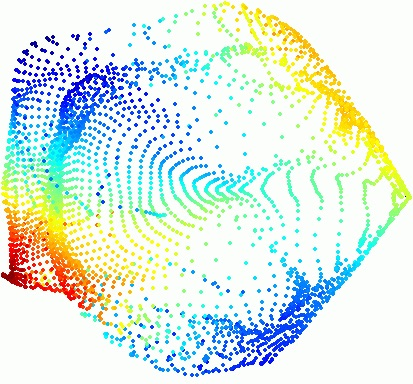
\includegraphics[width=5cm]{highD}
	\end{figure}
	Denote these $x_i \in \mathbb{R}^m$ for $i = 1...n$.
	\end{frame}
	
		\begin{frame}
			\frametitle{Representation and Factorization}
			We can \textit{approximate} $X \in \mathbb{R}^{n \times m}$.
		
			\only<1>{\begin{figure}
				\centering
				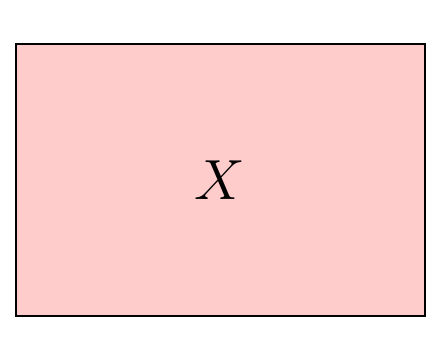
\includegraphics[height=3cm]{X}
			\end{figure}
			with rank$(X) = \min(m,n)$.}
			\only<2>{\begin{figure}
					\centering
					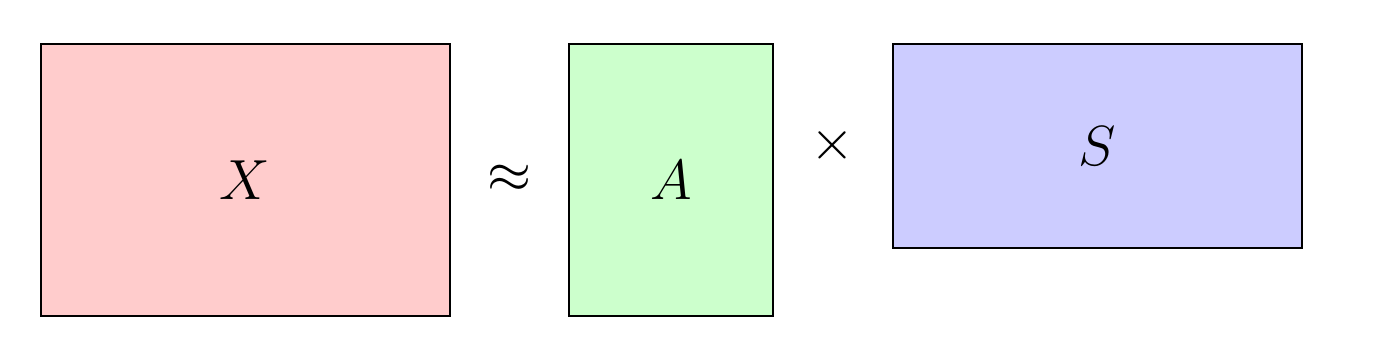
\includegraphics[height=3cm]{nnmf}
				\end{figure}
				with rank$(AS) = k << min(m,n)$.}
		\end{frame}
		
			\begin{frame}
				\frametitle{Low Dimensional Interpretation }
				Our original high-dimensional points are linear combinations of ``basis elements'.'
				$$X_i = \sum_{j=1 }^k A_{i,j} S_j$$
				
		\only<2>{\begin{figure}
						\centering
						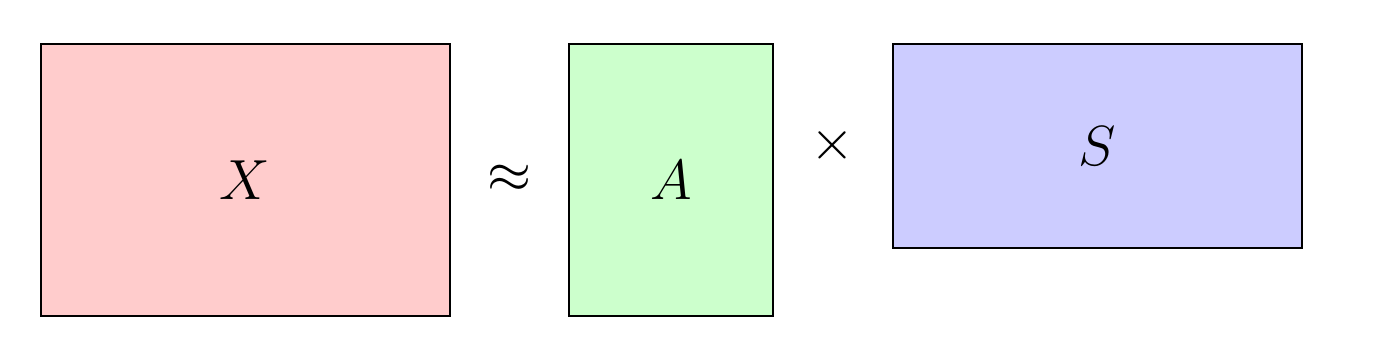
\includegraphics[height=3cm]{nnmf}
					\end{figure}}
					\onslide<3->{\begin{figure}
							\centering
							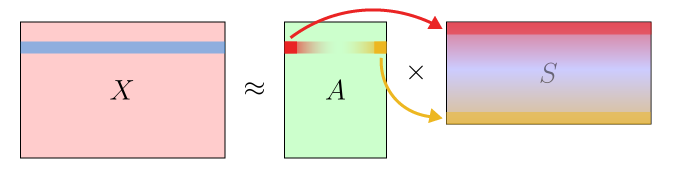
\includegraphics[height=3cm]{nnmfLC}
						\end{figure}}
					\only<4>{Find factorization by solving optimization problem $$\min_{A,S} ||X-AS||$$}.
			\end{frame}
			
			\begin{frame}
						\frametitle{Example (Lee and Seung 1999)}
					\onslide+<2->{
					A 19x19 pixel greyscale image of a face is a data point ($x_i \in \mathbb{R}^{361}$ with values between 0 and 256)}
				\onslide+<3->{	\begin{figure}
						\centering
						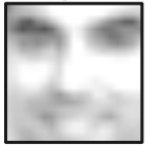
\includegraphics[height=3cm]{face}
					\end{figure} }
									\onslide+<4>{Take a database of 2,429 faces to get $X \in \mathbb{R}^{2429 \times 361}$}
					\end{frame}
					
							\begin{frame}
								\frametitle{Example (Lee and Seung 1999)}
							\onslide<1->{\textbf{Before:} Find any $A$ and $S$ such that $||X-AS||$ is minimized.
								\begin{figure}
									\centering
									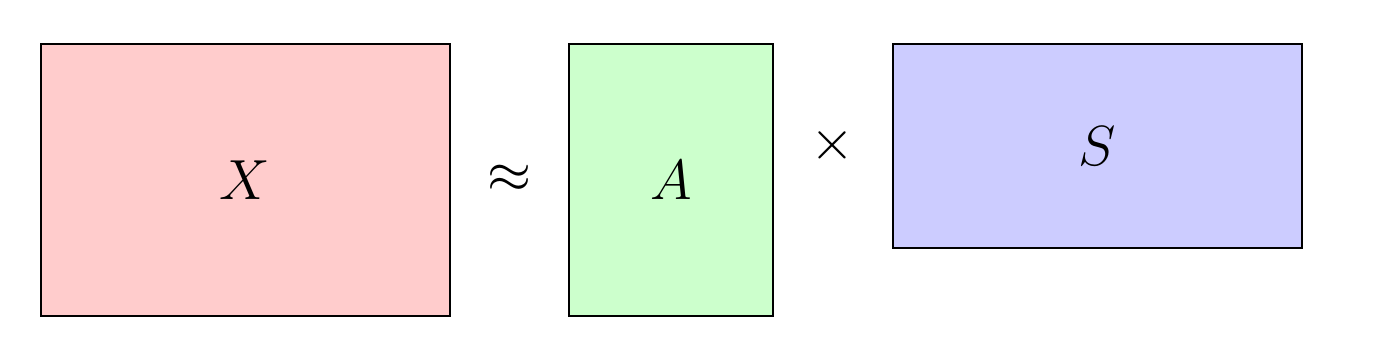
\includegraphics[height=2cm]{nnmf}
								\end{figure}}
								\onslide<2->{\textbf{Now:} We add some constraints 
									\begin{enumerate}
										\onslide<3->{\item Columns of $A$ to be orthonormal; Rows of $S$ to be orthogonal (PCA)}
										\onslide<4->{\item Row of $A$ sums to 1, which one entry equal to one and the rest equal to zero (VQ) }
										\onslide<5->{\item All entries of $A$ and $S$ are non-negative (NNMF)}
									\end{enumerate}}
										\onslide<6->{For each, find $A$ and $S$ subject to constraints that minimize 
											$$||X-AS||$$}
								\end{frame}
									\begin{frame}
										\frametitle{Example (Lee and Seung 1999)}
											\onslide<2->{\begin{figure}
													\centering 1: PCA
													\onslide<3->{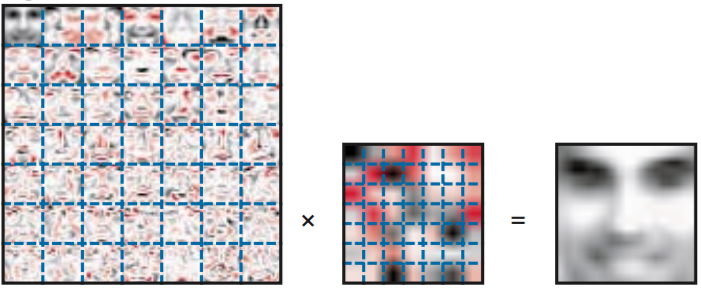
\includegraphics[height=2.4cm]{pcaFACE}}\onslide<4->{``eigenfaces''}
												\end{figure}}
										\onslide<5->{\begin{figure}
												\centering 2: VQ
											\onslide<6->{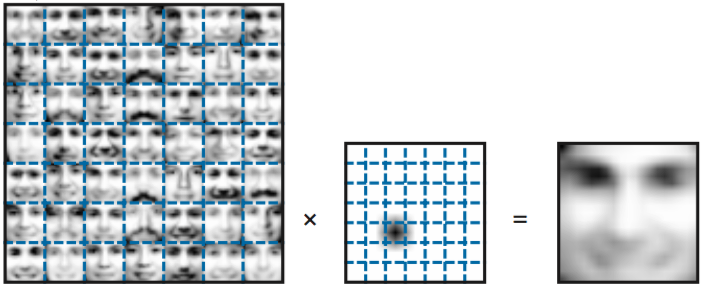
\includegraphics[height=2.4cm]{vqFACE}}		\onslide<7->{``protofaces''}
											\end{figure}}
										
												\onslide<8->{\begin{figure}
														\centering 3: NMF
														\onslide<9->{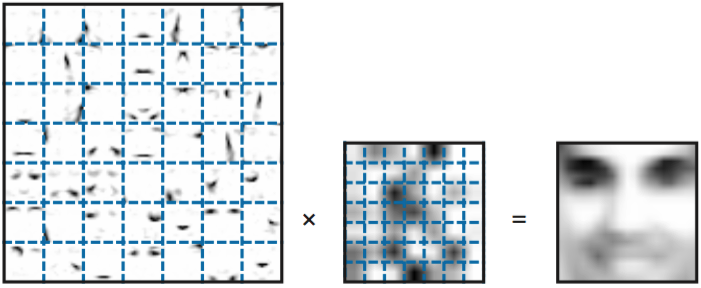
\includegraphics[height=2.4cm]{nmfFACE}}
														\onslide<10->{parts-based}
													\end{figure}}
										\end{frame}
												\begin{frame}
													\frametitle{Recognition-by-parts}
													NNMF learns an additive, parts based model
														\only<2>{\begin{figure}
														\centering
													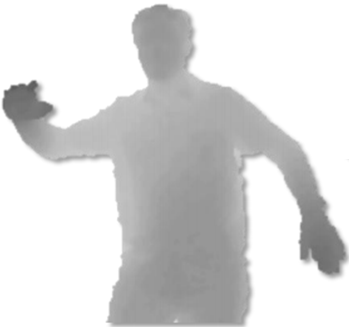
\includegraphics[height=2.4cm]{dingusBefore}
															\end{figure}}
													
														\only<3>{\begin{figure}
																\centering
																
\includegraphics[height=2.4cm]{dingus}
																\end{figure}
																	which is what our brain does when recognizing images!}
															
													
													\end{frame}
\end{document}